\documentclass[12pt]{article}

\author{Jonah Miller\\
\textit{jonah.maxwell.miller@gmail.com}}
\title{2+1-dimensional Fixed Boundaries CDT: Programmer's Guide}

\usepackage{fullpage}
\usepackage{verbatim}
\usepackage{listings}
\usepackage{color}
\usepackage{hyperref}
\usepackage{graphicx}
%\usepackage{algorithmic}

\begin{document}
\maketitle

\section{Introduction}
\label{s:intro}

This is the fixed boundaries branch of Rajesh Kommu's CDT code. The
algorithm was originally worked on by David Kemansky, and later
improved upon and updated by Jonah Miller.

The code implements CDT using an updated action that includes the
boundary terms.

The goal of this file is to explain how to modify the code. I will
first give some tips about lisp. Then I will present a very brief
overview of the algorithm of the program. Then dive into data
structures and specific functions and how they should be used. This
document assumes the reader knows how to run the program, its basic
structure, and the physics behind it. In order these can be found in:
\begin{itemize}
\item The user's guide.
\item The file called program\_and\_module\_list.txt
\item Ambj\o rn and Loll's ``Dynamically Triangulating Lorentzian
  Quantum Gravity,'' the documentation file
  ``Gibbons-Hawkin\_Boundary\_Term\_in\_Causal\_Dynamical\_Triangulations.pdf,''
  and my REU write-up.
\end{itemize}
All of these should be bundled in with the software in the
documentation folder.

Hopefully this guide will help elucidate how to edit the CDT
code-base. If you have any questions, don't hesitate to email me.

\section{Lisp Tips and Tricks}
\label{s:lisp:tricks}
\subsection{Common Lisp Implementations}

Although it is a programming language, ANSI Common Lisp is not a
single program. Rather, it is a set of guidelines about how the
programming language should behave. For this reason, there are a
number of different implementations of Common Lisp, all of which
behave slightly differently. We use Steel Bank Common Lisp, which can
be found here:
\begin{verbatim}
http://www.sbcl.org/
\end{verbatim}

\subsection{Resources}
Some resources on Lisp are:
\begin{itemize}
\item Peter Siebel's ``Practical Common Lisp'' is an excellent,
  readable, and in-depth guide to writing code in lisp. It was my
  primary resource and you can find it online.
  \begin{verbatim}
http://www.gigamonkeys.com/book/
\end{verbatim}
\item The canonical work on Lisp is Paul Graham's ``On Lisp.'' It is available online.
\begin{verbatim}
http://www.paulgraham.com/onlisp.html
\end{verbatim}
\item Successful Lisp is another book available for free online.
\begin{verbatim}
http://psg.com/~dlamkins/sl/contents.html
\end{verbatim}
\item This website links to a number of useful resources.
  \begin{verbatim}
http://www.apl.jhu.edu/~hall/lisp.html
\end{verbatim}
\end{itemize}
\subsection{Coding Tools}
\label{s:lisp:tools}
When I edit lisp, I use the emacs text editor with SLIME, a module for
emacs. This is not the only choice, but I think it is a very good one,
and I suspect it is the canonical choice. You can find the home
project for emacs here:
\begin{verbatim}
http://www.gnu.org/software/emacs/
\end{verbatim}
and the home project for slime here:
\begin{verbatim}
http://common-lisp.net/project/slime/
\end{verbatim}
For most Linux distributions, emacs and slime should be very easy to
install if you have administrator privileges. The following tutorial explains how to get a nice set up in ubuntu:
\begin{footnotesize}
\begin{verbatim}
https://functionalrants.wordpress.com/2008/09/06/how-to-set-up-emacs-slime-sbcl-under-gnulinux/
\end{verbatim}
\end{footnotesize}
If you don't have administrator access, see pages 1--8 in the document
labeled \textbf{cdthowto.pdf}. You may have to change some of the
version numbers to get everything working.\footnote{The rest of the
  cdthowto.pdf document is somewhat outdated. You're better off
  referring to the other documentation.}

Emacs is a complicated piece of software. A good online tutorial is
here:
\begin{verbatim}
http://www2.lib.uchicago.edu/keith/tcl-course/emacs-tutorial.html
\end{verbatim}
and Emacs includes a very good in-program tutorial as well. If you want to learn (much) more about what Emacs is capable of, check out ``Emacs Rocks'' and ``Emacs-Fu,'' two blogs about emacs:
\begin{verbatim}
http://emacsrocks.com/
http://emacs-fu.blogspot.com/
\end{verbatim}
Finally, a very good resource on emacs is the Emacs Wiki:
\begin{verbatim}
http://emacswiki.org/
\end{verbatim}

\subsection{Tips and Tricks}

When editing the CDT code, I suggest that you test your changes live,
as you write code. You can do this by running slime from within
emacs. Once you've opened up a *.lisp file, type ``Escape'' and then
``x'' to access a command prompt. Then type ``slime'' and press
``Enter.'' You will get a live Lisp interpreter. This is the ``REPL,''
which stands for
\textbf{R}ead-\textbf{E}val-\textbf{P}rint-\textbf{L}oop. Lisp is
compiled, not interpreted. However, compilation happens at runtime:
there is no separate compile-time step. One advantage of this is that
functions can be defined and byte-compiled during a runtime
algorithm. Another advantage is that you can prototype functions in
Lisp the same way you would for a scripting language like
Python. Indeed, you can do more than that, you can initialize a
spacetime, and then define or redefine functions live and call them in
the simulation to see what they do. While editing a *.lisp file with
slime, if the REPL is active, you can compile a function by pressing
``C-c C-c.'' This is how I suggest you change your code.

\section{The Algorithm}
\label{s:algorithm}
Although I'm sure the reader is familiar with the algorithm of CDT, I
present it here for completeness. The metropolis algorithm as applied
to CDT is as follows:
\begin{enumerate}
\item Generate an arbitrary spacetime constructed of equilateral simplices.
\item Randomly apply one of the ergotic moves to the spacetime.
\item Calculate whether the new spacetime is more or less likely than
  the old spacetime, or less, as given by its un-normalized weight in
  the partition function,\footnote{Technically, the normalized weight
    $\frac{1}{Z}e^{iS}$ is the important quantity. However, since we
    only care about the ratio of weights, the factor of $1/Z$ cancels
    out. This is fortunate, since we don't know what $Z$ is---if we
    did, we could simply perform the path integral.} $e^{i S}$.
\item If the new spacetime is more likely than the previous spacetime,
  accept the change with probability $P=1$. If it is less likely,
  accept the change with probability $P = P(new)/P(old)$. We can
  rewrite this probability as
  $$P = e^{i S_{new} - i S_{old}}.$$
\item Return to step 2, and repeat until the spacetime is acceptably
  probable.
\end{enumerate}
The primary data structures we need to worry about, then, are the
geometric objects. These, and the functions that manipulate them, will
be discussed in section \ref{s:data-structures}. The most important
functions are the action and the ergotic moves. These will be
discussed in some detail in section \ref{s:functions}.

\section{Data Structures}
\label{s:data-structures}

The most important data structures in the simulation are, of course
the goemetric objects that make up the spacetimes. These are points,
edges, triangles, and tetrahedra. 

The other important data structures in the simulation are the f- and
b-vectors, which count geometric objects. We will discuss these after
we discuss the geometric objects.

\subsection{Points}
\label{ss:points}

Points are represented as integer identifiers. There is no master list
of points, but, whenever a new point is created, the value of a global
variable is incremented to obtain the next point ID. Points have no
coordinates in this program. In some sense, points are the most
important objects in the simulation. As will be discussed below, the
higher-dimensional simplices are partly defined by which points they
contain. Objects that manipulate points are:
\lstset{language=Lisp,frame=shadowbox,rulesepcolor=\color{blue}}
\begin{itemize}
\item \textbf{*LAST-USED-POINT*}---This is the global variable that is
  incremented to obtain point ids. It starts at 0.
\item \textbf{next-pt}---This is a function that increments
  *LAST-USED-POINT* by 1. It then returns the incremented
  *LAST-USED-POINT*. Call it with
\begin{lstlisting}
(next-pt)
\end{lstlisting}
Thus, 
\begin{lstlisting}
(format t "The next point is ~A~%." (next-pt))
\end{lstlisting}
would return 
\begin{verbatim}
The next point is <next point>.
\end{verbatim}
\item \textbf{set-last-used-pt}---In certain circumstances, for
  instance when loading a spacetime from file, we just want to tell
  the simulation how many points IDs have been used, rather than
  increment the global variable. The call
\begin{lstlisting}
(set-last-used-pt point-number)
\end{lstlisting}
will set *LAST-USED-POINT* to point-number.
\end{itemize}

*LAST-USED-POINT* and all objects that manipulate it can be found in ``globals.lisp.''

\subsection{Links/Edges}
\label{s:links-edges}
Links are the edges of tetrahedra. There can be time-like links which
connect points at two different times and space-like links which
connect points at the same time. Since they are one dimensional, we
also call links 1-simplices. Links, faces, and tetrahedra are stored
in hash tables.\footnote{A hash table is a generalized list. You can
  think of it as a function in the mathematical sense: It maps a
  \textit{key} to a \textit{value}.} 

Space-like links are stored in the hash table named
\begin{lstlisting}
*SL1SIMPLEX->ID*
\end{lstlisting}
and time-like links are stored in the hash table named
\begin{lstlisting}
*TL1SIMPLEX->ID*
\end{lstlisting}

As the name implies, the key of the hash table contains the geometric
object itself. The value associated with each key is actually just
0. For the lower-dimensional simplices, only the keys are really
used. Because hash tables can be thought of like mathematical
functions, a given key can't be entered into the hash table twice---it
just doesn't make sense. If I tried to add a new entry to the hash
table that shared a key with an existing entry, the value of the
existing entry would be overwritten, but otherwise nothing would
change. By storing geometric information in the keys of a hash table,
we ensure that we have no duplicate geometric objects.

All 1-simplices contained in a given 3-simplex can be generated with
the command \textbf{make-1simplices}, which has the following prototype:
\begin{lstlisting}
(defun make-1simplices (sxtype tmlo tmhi p0 p1 p2 p3)
\end{lstlisting}
The inputs here are relevant data from the definition of a 3-simplex,
which I will discuss more below. sxtype is the type of
tetrahedron---(2,2), (3,1), or (1,3)---; tmlo and tmhi are the time
slices the simplex spans; and p0,p1,p2,p3 are the points of the
simplex.

\subsubsection{An Aside on Generating Lower-Dimensional Simplices}
I will discuss each hash table for these objects in a little bit more
detail below, but before I do that, I want to discuss how these
objects, and objects like them, are usually generated. In general,
lower-dimensional simplices are created when the higher-dimensional
simplices are created. In other words, the function make-3simplex will
generate the lower-dimensional subsimplices as a matter of course.

The upside of this is that a programmer usually doesn't have to worry
about explicitly keeping track of these simplices---lower-level
functions are already doing all the book-keeping. However, an easy
trap to fall into is to forget to remove lower-dimensional
simplices. Removing a 3-simplex does not necessarily remove
constituent sub-simplices, since that 3-simplex almost certainly
shares some of its subsimplices with other simplices (in fact it
always will). For this reason, lower-dimensional simplices are
generated automatically by lower-level functions, but the programmer
must intentionally remove them.

\subsubsection{*SL1SIMPLEX-$>$ID*}
\label{sss:sl1simplex:id}
The keys for the *SL1SIMPLEX-$>$ID* hash table are of the form:
\begin{lstlisting}
(tslice (p0 p1))
\end{lstlisting}
where tslice is the proper time the edge lives in, or the time slice
that contains the edge, and p0 and p1 are the endpoints of the
edge. The parentheses represent that the key is a list. (p0 p1) is
another list. As discussed at the beginning of section
\ref{s:links-edges}, the value for each entry in the hash table is
\textbf{0}.

You can remove spacelike 1-simplices with the commands
\textbf{remove-sl1simplex} and \textbf{remove-sl1simplices}, which
have the prototypes
\begin{lstlisting}
(defun remove-sl1simplex (sl1sx))
\end{lstlisting}
and 
\begin{lstlisting}
(defun remove-sl1simplices (sl1sxs))
\end{lstlisting}
respectively. The former accepts a single simplex key. The second
accepts a list of simplices.

You can look at the entire hash table with the function
\textbf{show-sl1simplex-store}, with prototype
\begin{lstlisting}
(defun show-sl1simplex-store ())
\end{lstlisting}
and function call
\begin{lstlisting}
(show-sl1simplex-store)
\end{lstlisting}

You can access the spacelike links at a given time with the function
\textbf{get-spacelike-links-at-time}, which has the
prototype\footnote{When I describe prototypes, the prototype itself
  probably doesn't exist, since this program doesn't prototype
  functions. However, the prototype gives the user the relevant
  information about a function call.}
\begin{lstlisting}
(defun get-spacelike-links-at-time (t0))
\end{lstlisting}
and you can count the number of spacelike links at a given time with
the function \textbf{count-spacelike-links-at-time}, which has the
prototype
\begin{lstlisting}
(defun count-spacelike-links-at-time (t0))
\end{lstlisting}
and you can count the spacelike 1simplices in the entire spacetime
with the function \textbf{count-spacelike-links-in-spacetime}, which
has the prototype
\begin{lstlisting}
(defun count-spacelike-links-in-spacetime ()).
\end{lstlisting}

\subsubsection{*TL1SIMPLEX-$>$ID*}
\label{sss:tl1simplex:id}

The keys for the *TL1SIMPLEX-$>$ID* hash table are of the form:
\begin{lstlisting}
(t_low t_high (p0 p1))
\end{lstlisting}
where t\_low and t\_high are the proper times between which the link
is suspended, and p0 and p1 are the endpoints of the edge. As
discussed at the beginning of section \ref{s:links-edges}, the value
for each entry in the hash table is \textbf{0}.

You can remove timelike 1-simplices with the commands
\textbf{remove-tl1simplex} and \textbf{remove-tl1simplices}, which
have the prototypes
\begin{lstlisting}
(defun remove-tl1simplex (tl1sx))
\end{lstlisting}
and 
\begin{lstlisting}
(defun remove-tl1simplices (tl1sxs))
\end{lstlisting}
respectively. The former accepts a single simplex key. The second
accepts a list of simplices.

You can look at the entire hash table with the function
\textbf{show-tl1simplex-store}. The function call is analogous to that
for show-sl1simplex-store. You can access the spacelike links at a
given time with the function \textbf{get-timelike-links-in-sandwich},
which has the prototype
\begin{lstlisting}
(defun get-timelike-links-in-sandwich (t-low t-high))
\end{lstlisting}
and you can count the number of spacelike links at a given time with
the function \textbf{count-timelike-links-in-sandwich}, which has the
prototype
\begin{lstlisting}
(defun count-timelike-links-in-sandwich (t-low t-high))
\end{lstlisting}
and you can count the spacelike 1simplices in the entire spacetime
with the function \textbf{count-timelike-links-in-spacetime}, which
has the prototype
\begin{lstlisting}
(defun count-timelike-links-in-spacetime ()).
\end{lstlisting}

You probably noticed that the spacelike and timelike 1simplices had
very similar behavior and functions. This parallel will continue with
spacelike and timelike triangles (also known as faces or 2-simplices).

\subsection{Triangles/Faces}
\label{s:data:tetrahedra}
Triangles are the faces of the tetrahedra that make up a
spacetime. Since they are two-dimensional, we also call them
2-simplices or 2simplices. Space-like triangles are stored in the hash
table named
\begin{lstlisting}
*SL2SIMPLEX->ID*
\end{lstlisting}
and time-like triangles are stored in the hash table named
\begin{lstlisting}
*TL2SIMPLEX->ID*
\end{lstlisting}

As with the edges, the hash table key contains the geometric object
itself, and the value is \textbf{0}. All 2-simplices contained in a
given 3-simplex can be generated with the \textbf{make-2simplices}
function, which has the following prototype:
\begin{lstlisting}
(defun make-2simplices (sxtype tmlo tmhi p0 p1 p2 p3))
\end{lstlisting}
The function takes the same inputs as make-1simplices.

\subsubsection{*SL2SIMPLEX$->$ID*}
The keys for the *SL2SIMPLEX$->$ID* hash table are of the form
\begin{lstlisting}
(tslice (p0 p1 p2))
\end{lstlisting}
where tslice is the time slice the triangle lives in and p0, p1,and p2
are the vertices of the triangle. Just like in the 1-simplex case, the
value for a given key is always 0. 

You can remove space-like 2-simplices with the commands
\textbf{remove-sl2simplex} and \textbf{remove-sl2simplices}, which
have prototypes and function calls analogous to the matching functions
for space-like and time-like 1-simplices. You can access the
space-like triangles with \textbf{show-sl2simplex-store}. You can
access the spacelike triangles at a given time with
\textbf{get-spacelike-triangles-at-time}, and you can count them with
\textbf{count-spacelike-triangles-at-time} and
\textbf{count-spacelike-triangles-in-spacetime}. The prototypes and
function calls are analogous to those for the functions for space-like
1-simplices.

There is an additional function, \textbf{3sx2p1$->$s2sx2p1}, with the
prototype
\begin{lstlisting}
(defun 3sx2p1->s2sx2p1 ())
\end{lstlisting}
which fills a hash table
\begin{lstlisting}
*ID->SPATIAL-2SIMPLEX*
\end{lstlisting}
with information on space-like 2-simplices as a function of proper
time. At each proper time, the points and simplices will be numbered
in such a way that the time slice will describe a surface in a
coordinate-free way. I have never used this function, but I believe
Rajesh uses it for data analysis. You can find this function and many
more functions to do with spatial simplices in the module
\textbf{spacelike\_2simplices.lisp}.


\subsubsection{*TL2SIMPLEX$->$ID*}
The keys for the *TL2SIMPLEX$->$ID* hash table are of the form
\begin{lstlisting}
(type tmlo (p0 p1 p2))
\end{lstlisting}
where the type is an integer, type$\in\{1,2\}$. It represents whether
a triangle has one vertex in the lower time slice, or two
(respectively). tmlo is the lower time slice that the the triangle is
connected to. p0, p1, and p2 are the vertices of the triangle. The
first type vertices are in the lower time slice and the last $3-$type
vertices are in the upper time slice. Just like in the 1-simplex case,
the value for a given key is always 0.

As before, you remove time-like 2-simplices with the commands
\textbf{remove-tl2simplex} and \textbf{remove-tl2simplices}. You can
access the triangles with \textbf{show-tl2simplex-store},
\textbf{get-timelike-triangles-in-sandwich}, and you can count them
with \textbf{count-timelike-triangles-in-sandwich} and
\textbf{count-timelike-triangles-in-spacetime}. The prototypes and
calls are analogous to those for time-like 1-simplices.

\subsection{Tetrahedra/3-simplices}
Tetrahedra are the highest-level simplices in the spacetime. These are
the most important objects: those changed by the ergotic moves. They
are also by far the most complicated data structure in the
program. There are three types of tetrahedra, labeled by the number of
points in the lower time slice of the two slices they span:
type$\in\{1,2,3\}$. A type 1 tetrahedron is a $(1,3)$-simplex. A type
2 tetrahedron is a $(2,2)$-simplex, and a type 3 tetrahedron is a
$(3,1)$-simplex. Tetrahedra are stored in the hash table
\begin{lstlisting}
*ID->3SIMPLEX*
\end{lstlisting}
and it uses both keys and values.

The key is a numeric ID number assigned when the simplex is
created. The 3-simplex IDs are generated in much the same way as the
point IDs are generated. The programmer can find the functions
\textbf{next-3simplex-id} and \textbf{recycle-3simplex-id} in the file
globals.lisp. \textbf{recycle-3simplex-id} fulfills a special
purpose. When a simplex is removed from the spacetime, its ID is added
to a list \textbf{*RECYCLED-3SX-IDS*}. Later, when we want a new ID,
\textbf{next-3simplex-id} first checks the list of recycled IDs and
takes an element of that list. If the list is empty, then a new ID is
generated. If we don't do this, the number of IDs and their values
quickly becomes completely intractable.

The value of \textbf{*ID$->$3SIMPLEX*} is the geometric object in
question. The object is defined as
\begin{lstlisting}
(sxtype tmlo tmhi (p0 p1 p2 p3) (n1 n2 n3 n4))
\end{lstlisting}
where sxtype is the type of 3-simplex, as discussed at the beginning
of \ref{s:links-edges}, tmlo and tmhi are the indexes of the
time slices that the simplex spans. p0, p1, p2, p3 are the vertices of
the tetrahedron, and the first type of them are in the lower time
slice. n1, n2, n3, and n4 are the neighbors of the simplex---The ids
of the tetrahedra that share a face with this tetrahedron. They are
ordered such that the neighbor attached to the tetrahedron at the face
opposite p1 is n1, the neighbor attached at the face opposite p2 is
n2, etc..

When a simplex is created \textbf{make-3simplex} (more on that below),
the neighbor ids are all set to zero. The neighbors are set later
using the command \textbf{connect-3simplices} and derivative
functions. The reason for this is that the neighbors will be modified
as the spacetime manifold changes. I will first describe simplex
creation, then connecting neighbors, and then I will name the
functions that access 3-simplices, which are often quite similar to
the functions for lower-dimensional simplices.

\subsubsection{Generation}
The core function here is \textbf{make-3simplex}. It has the prototype 
\begin{lstlisting}
(defun make-3simplex (sxtype tmlo tmhi p0 p1 p2 p3))
\end{lstlisting}
and takes simplex type, time slices, and point IDs as its input. It
doesn't take in neighbor IDs, because neighbor IDs are set later. This
is the lowest-level tetrahedron function, and it generates
sub-simplices automatically by calling make-2simplices and
make-1simplices. It returns the ID number of the simplex, which it
generates using next-3simplex-id. 

There are also a number of functions that call make-3simplex for
specialized purposes. \textbf{make-3simplex-v2} takes only 4 inputs,
since the points are ``packed'' into a list. It's used when the
ergodic moves are applied, since it is tailor-made to take the output
of the try-move functions (more on these later) as input. The function
definition is:
\begin{lstlisting}
(defun make-3simplex-v2 (sxtype tmlo tmhi pts)
    (let ((p0 (nth 0 pts))
	(p1 (nth 1 pts))
	(p2 (nth 2 pts))
	(p3 (nth 3 pts)))
    (make-3simplex sxtype tmlo tmhi p0 p1 p2 p3)))
\end{lstlisting}
\textbf{make-3simplex-v3} is only used during the space-time
initialization part of the algorithm. If periodic boundary conditions
are specified, it adjusts the points on the final and initial
time-slices, since the $t=t_{final}$ time slice is identified with the
$t=0$ time slice. It also sets the variable *LAST-USED-POINT*, which
is required for algorithm for fixed boundary
conditions. \textbf{make-3simplex-v4} is used when loading a spacetime
from a file, because the input is slightly
different. \textbf{make-3simplex-v5} takes a single list as input,
where the list contains all simplex data. A function call might look like
\begin{lstlisting}
(make-3simplex-v5 (list sxtype tmlo tmhi (list p0 p1 p2 p3)))
\end{lstlisting}
it is primarily used in the function
\textbf{make-3simplices-in-bulk}. \textbf{make-3simplices-in-bulk} is
used when applying a move, specifically in the function
\textbf{2plus1move}, which will be described later. It takes a list of
inputs to make-3simplex-v5. The function definition is
\begin{lstlisting}
(defun make-3simplices-in-bulk (simplex-data-list)
  (let ((3sxids nil))
    (dolist (simplex-data simplex-data-list)
      (push (make-3simplex-v5 simplex-data) 3sxids))
    3sxids))
\end{lstlisting}

Since 3-simplices start with no neighbors defined, we have to set
their neighboring simplices using \textbf{connect-3simplices}. This
function takes two 3-simplex IDs as input and, if they are neighbors,
modifies their values in the hash table accordingly. This means
finding which face they share (defined by the point opposite that
face) and modifying the element of the list of neighbors corresponding
to that point.

We connect only a few 3-simplices at a time rather than connecting all
simplices in the spacetime for efficiency reasons. We only need to
connect a few simplices in the region of the spacetime we changed, so
we don't want to check the entire spacetime each time. We have some
functions that let us selectively connect more than two
simplices. \textbf{connect-3simplices-within-list} takes a list of
3-simplex ids and runs connect-3simplices on every possible
combination of 3-simplices in the
list. \textbf{connect-3simplices-across-lists} takes two lists of
3-simplex ids as input, and tries to connect every 3-simplex in the
first list with every 3-simplex in the second list. However, it
doesn't try to connect 3-simplices in the first list with other
3-simplices in the first list. \textbf{3simplices-connected?} takes 2
simplex IDs as input. If they're listed as neighbors in each-others'
list of neighbors, it returns true. Otherwise, it returns false.

\subsubsection{Access}
\label{s:d:tetrahedra:access}
Because the 3-simplex data structure is used so often, and because it
is somewhat complicated, there are some macros designed to make the
code more readable when accessing 3-simplices. They are:
\begin{small}
\begin{lstlisting}
(defmacro 3sx-type (sx) `(first ,sx))
(defmacro 3sx-tmlo (sx) `(second ,sx))
(defmacro 3sx-tmhi (sx) `(third ,sx))
(defmacro 3sx-points (sx) `(fourth ,sx))
(defmacro 3sx-sx3ids (sx) `(fifth ,sx))
(defmacro 3sx-lopts (sx) `(subseq (3sx-points ,sx) 0 (3sx-type ,sx)))
(defmacro 3sx-hipts (sx) `(subseq (3sx-points ,sx) (3sx-type ,sx)))
(defmacro nth-point (sx n) `(nth ,n (3sx-points ,sx)))
(defmacro nth-neighbor (sx n) `(nth ,n (3sx-sx3ids ,sx)))
\end{lstlisting}
\end{small}
each takes a 3-simplex geometric object, not its id. An easy way to
get a simplex associated with a given id is \textbf{get-3simplex},
which takes an ID as input, and returns the simplex geometric
object. 

\textbf{remove-3simplex} and \textbf{remove-3simplices} remove
tetrahedra from their hash table and take as inputs 3-simplex ID and a
list of IDs respectively. \textbf{show-id->3simplex-store} outputs the
hash table for tetrahedra in a human-readable way. It takes no input. 

3-simplices are defined by their type and by the pair of time-slices
they are sandwiched between. Thus the functions that access them are
written with this in mind. \textbf{get-simplices-in-sandwich} has the
prototype
\begin{lstlisting}
(defun get-simplices-in-sandwich (tlo thi))
\end{lstlisting}
where tlo is the lower time slice and thi is the upper time slice that
``sandwich'' a bunch of tetrahedra. This function returns a list of IDs of
all tetrahedra times in the
sandwich. \textbf{get-simplices-in-sandwich-of-type}, on the other
hand, returns only 3-simplices of the given type. It has prototype
\begin{lstlisting}
(defun get-simplices-in-sandwich-of-type (tlo thi typ))
\end{lstlisting}
where typ$\in\{1,2,3\}$ and indexes 3-simplex types as described in
the beginning of section
\ref{s:links-edges}. \textbf{get-simplices-in-sandwich-ordered-by-type}
is like get-simplices-in-sandwich, but it orders them from type 1 to
type 3. \textbf{get-simplices-of-type} takes a type integer as input
and returns all 3-simplices of that
type. \textbf{count-simplices-of-type} and
\textbf{count-simplices-in-sandwich} work like their corresponding
``get'' functions, but they return integers rather than lists of
simplex ids. \textbf{count-simplices-of-all-types} does exactly what
it says on the can. It takes no inputs.

A function unique to fixed-boundaries CDT is
\textbf{count-boundary-vs-bulk}. It takes no input and returns a list
of the number of simplices of various and various locations. The
output looks something like this
\begin{lstlisting}
(N13-INITIAL-SLICE N22-INITIAL-SLICE N31-INITIAL-SLICE
 N13-BULK N22-BULK N31-BULK
 N13-FINAL-SLICE N22-FINAL-SLICE N31-FINAL-SLICE
 N3-TOTAL)
\end{lstlisting}
where N13-INITIAL-SLICE, N22-INITIAL-SLICE, and N31-INITIAL-SLICE are
the number of $(1,3)$-simplices, $(2,2)$-simplices, and
$(3,1)$-simplices respectively in the time slice defined by
$t=0$. Analogously, N13-BULK, N22-BULK, and N31-BULK are the simplices
in the bulk of the spacetime and N13-FINAL-SLICE, N22-FINAL-SLICE, and
N31-FINAL-SLICE are the simplices in the time slice defined by
$t=t_{final}$. N3-TOTAL is the total number of 3-simplices in the
space time.

There are a number of macros that test a 3-simplex's position in the
spacetime manifold. \textbf{in-upper-sandwich} takes an ID number. If
the boundary conditions are open and the simplex with the given ID has
tmlo=t\_max-1 and tmhi=t\_max, then the macro returns true. Otherwise,
it returns false. \textbf{in-lower-sandwich} works like
in-upper-sandwich, but returns true if tmlo=0 and
tmhi=1. \textbf{in-either-boundary-sandwich} returns true if either
in-upper-sandwich or in-lower-sandwich returns
true. \textbf{has-face-on-boundary} takes the ID of a 3-simplex as
input and returns true of that 3-simplex has one face contained in
either the initial or the final time slice. Obviously this macro
always returns false for $(2,2)$-simplices.

\subsubsection{Generic Counting Functions}

A number of the functions that count and list geometric objects are
actually calls of the metafunctions contained in
\textbf{generalized-hash-table-counting-functions.lisp}. These are
worth discussing in some detail, since they could save a lot of time,
if you need to make new functions that interact with hash tables. We
discuss them here, rather than in the functions section, because they
are closely related to the data structures discussed in this
section. Let's look at \textbf{list-keys-with-trait}:
\begin{lstlisting}
(defun list-keys-with-trait (trait hashtable key-subindex)
  (let ((keylist nil)
	(vallist nil))
    (flet ((discriminator (hkey hval)
	     (when (funcall trait (nth key-subindex hkey))
	       (push hkey keylist)
	       (push hval vallist))))
      (maphash #'discriminator hashtable)
      keylist)))
\end{lstlisting}
trait is a function that returns a Boolean value. hashtable is the
hash table we're interested in acquiring keys from. key-subindex is an
integer. These functions assume the key is a geometric object, and
that the keys are lists. Thus, key-subindex is the index of the list
of the key that we want the trait function to act
on. list-keys-with-trait goes through hashtable and, for each entry,
texts whether or not the trait function returns true when it is
applied to the key-subindex'th element of the key. If it is, then that
entry of the hash table is added to the list keylist. The function
then returns keylist. As an example, if we wanted to list all the
space-like 2-simplices at time 0, the function call would be:
\begin{lstlisting}
(list-keys-with-trait #'(lambda (x) (= x 0)) *SL2SIMPLEX->ID* 0)
\end{lstlisting}

\textbf{count-keys-with-trait} works like list-keys-with-trait, except
that it returns an integer, the number of keys where trait is
true. \textbf{list-vals-with-trait} and \textbf{count-vals-with-trait}
work like list-keys-with-trait and count-keys-with trait respectively,
except that they test the value of an entry in the hash table, rather
than the key.

Although they don't interact with hash tables, we do have two more
metafunctions designed to interact with our geometric
objects. \textbf{count-over-all-spacetime-slices} runs a function that
returns an integer as a function of time slice (like
count-points-at-time) and applies it to each time-slice and sums over
the results. \textbf{count-over-all-spacetime-sandwiches} works the
same as count-over-all-spacetime-slices, but accepts functions that
take two proper times (for a spacetime sandwich) as input, such abs
count-simplices-in-sandwich, as input.

\subsection{The f- and b-vectors}
\label{s:f-and-b-vectors}

The discrete Regge action depends on the number of simplices of
various type and dimension that make up the spacetime. The boundary
term depends on the number of simplices in the boundary, as opposed to
those in the bulk. We could, in theory, count up the number of
simplices in the spacetime after every move and see if action has
increased or decreased. However, this would be extremely slow and
memory-intensive, since we'd have to keep track of the spacetime
twice: once for before the move and once for after the move. We'd also
have to run the counting functions, which are slow, every time we
wanted to find out what the action was. A better way to predict
changes in the action is to count the number of simplices once at
initialization, and then simply keep track of how each ergodic move
changes the number of simplices of each type we care about: both in
the boundary and in the bulk. The f- and b-vectors do just that.

\subsubsection{The f-Vector}
The F-vector is defined as 
\begin{small}
\begin{displaymath}
  \vec{f} = \left[\begin{array}{c}N0\\N1-SL\\N1-TL\\N2-SL\\N2-TL\\
      N3-TL-31\\N3-TL-22\end{array}\right]
  = \left[\begin{array}{c}\texttt{The number of points in the spacetime}\\
      \texttt{The number of space-like edges in the spacetime}\\
      \texttt{The number of time-like edges in the spacetime}\\
      \texttt{The number of space-like triangles in the spacetime}\\
      \texttt{The number of time-like triangles in the spacetime}\\
      \texttt{The number of }(3,1)-\texttt{and }(1,3)-\texttt{simplices in the spacetime}\\
      \texttt{The number of }(2,2)-\texttt{simplices in the spacetime}\end{array}\right].
\end{displaymath}
\end{small}
Each element of the f-vector is its own variable that can be accessed
on its own. For instance, there is a macro to get the total number of
3-simplices in the spacetime:
\begin{lstlisting}
(defmacro N3 ()
  "total number of timelike 3simplices (tetrahedra)"
  `(+ N3-TL-31 N3-TL-22))
\end{lstlisting}
You can set the f-vector with the function \textbf{set-f-vector}:
\begin{lstlisting}
(defun set-f-vector (v1 v2 v3 v4 v5 v6 v7)
  (setf N0 v1 N1-SL v2 N1-TL v3 N2-SL v4
        N2-TL v5 N3-TL-31 v6 N3-TL-22 v7))
\end{lstlisting}
and you can print the current f-vector in a human-readable form with
the function \textbf{f-vector}.

You can update the f-vector with the function
\textbf{update-f-vector}, which takes a list as input, where the
$i^{th}$ element of the list is the change to the $i^{th}$ element of
the f-vector.

Each of the 5 ergodic moves changes the 5-vector the same way each
time it is applied to the spacetime. For this reason, changes to the
f-vector are defines as global variables so that they can be passed
directly to update-f-vector:
\begin{lstlisting}
(defparameter DF26 '(1 3 2 2 6 4 0))
(defparameter DF62 '(-1 -3 -2 -2 -6 -4 0))
(defparameter DF44 '(0 0 0 0 0 0 0))
(defparameter DF23 '(0 0 1 0 2 0 1))
(defparameter DF32 '(0 0 -1 0 -2 0 -1))
\end{lstlisting}
\textbf{DF26} is the change to the f-vector due to a 2-$>$6 move,
\textbf{DF23} is due to a 2-$>$3 move etc.. The DFnm variables are
returned by the try-move functions discussed below.

\subsubsection{The b-vector}

In addition to the f-vector, which keeps track of total information
(not bulk information), we also have the b-vector, which keeps track
of boundary information only. This is useful for fixed boundary
conditions. The b-vector is defined as:
\begin{small}
\begin{eqnarray}
  \vec{b}&=&\left[\begin{array}{c}\texttt{*}N1-SL-TOP*\\
      \texttt{*}N3-22-TOP*\\\texttt{*}N3-31-TOP*\\
      \texttt{*}N1-SL-BOT* \\\texttt{*}N3-22-BOT*\\ 
      \texttt{*}N3-31-BOT*\end{array}\right]\nonumber\\
  &=&\left[\begin{array}{c}\texttt{\# of space-like edges in the }t=t_{final}\texttt{ boundary}\\
      \texttt{\# of }(2,2)-\texttt{simplices with an edge in the }t=t_{final}\texttt{ boundary}\\
      \texttt{\# of }(3,1)-\texttt{and }(1,3)-\texttt{simplices with }\geq 1\texttt{ vertex in the }t=t_{final}\texttt{ boundary}\\
      \texttt{\# of space-like edges in } t=0\texttt{ boundary}\\
      \texttt{\# of }(2,2)-\texttt{simplices with an edge in the }t=0\texttt{ boundary}\\
      \texttt{\# of }(3,1)-\texttt{and }(1,3)-\texttt{simplices with }\geq 1\texttt{ vertex in the }t=0\texttt{ boundary}\end{array}\right]\nonumber
\end{eqnarray}
\end{small}
and it works much the same ways as the f-vector. Each element is its
own variable that can be called individually. You can set the b-vector
with the function \textbf{set-b-vector}, you can update the b-vector
with \textbf{update-b-vector}, and you can view the b-vector in
human-readable form with \textbf{b-vector}, which all work the same
way as the corresponding function for the f-vector.\footnote{Note that the indices of the b-vector do
  not at all correspond to the indices of the f-vector. The b-vector
  contains only the elements of the boundary required for the boundary
  term in the Regge action.}

Like with the f-vector, we keep track of how each ergodic move changes
the b-vector. However, the changes to the b-vector are dependent on
whether or not a move affects simplices in the boundary. For this
reason, the functions that change the b-vector are (almost)
all\footnote{The 4-$>$4 move never affects simplex counts, so it is
  just a constant.} macros that take a simplex ID as input, where that
simplex ID comes from the 3-simplex chosen to apply a move onto. The changes in the b-vector are:
\begin{lstlisting}
(defmacro DB23 (sxid) ; Change in b-vector due to 23-move.
  `(cond ((in-upper-sandwich ,sxid) (list 0 1 0 0 0 0))
	 ((in-lower-sandwich ,sxid) (list 0 0 0 0 1 0))
	 (t                         (list 0 0 0 0 0 0))))
\end{lstlisting}
\begin{lstlisting}
;; change in b-vector due to 32-move. Inverse of DB23
(defmacro DB32 (sxid) 
  `(cond ((in-upper-sandwich ,sxid) (list 0 -1 0 0 0  0))
	 ((in-lower-sandwich ,sxid) (list 0  0 0 0 -1 0))
	 (t                         (list 0  0 0 0  0 0))))
\end{lstlisting}
\begin{lstlisting}
(defparameter DB44 '(0 0 0 0 0 0)) ; Change in b-vector due to a
				   ; 44-move. 44 is its own inverse.
\end{lstlisting}
\begin{lstlisting}
(defmacro DB26 (sxid) ; Change in b-vector due to a 26-move.
  `(cond ((and (has-face-on-boundary ,sxid) *merge-faces*)
	  (list 3 0 2 3 0 2))
	 (t (list 0 0 0 0 0 0))))
\end{lstlisting}
\begin{lstlisting}
(defmacro DB62 (sxid) ; Change in b-vector due to a 62-move.
  `(cond ((and (has-face-on-boundary, sxid) *merge-faces*)
	  (list -3 0 -2 -3 0 -2))
	 (t (list 0 0 0 0 0 0))))
\end{lstlisting}

The variable \textbf{*merge-faces*} perhaps deserves some
description. If *merge-faces* is set to a non-nil value, and the
boundary conditions are set to ``OPEN,'' then the initial and final
boundaries will be identified, but the simulation will keep track of
changes to the boundary and put them into the action. This mode is
really only for debugging purposes and shouldn't be used for a real
simulation. All functions and variables relating to the f- and
b-vectors can be found in \textbf{tracking\_vectors.lisp}.


\section{Functions}
\label{s:functions}

We're now ready to talk about the primary functions in the
simulation. There are a number of broad categories of function that
interact with each other as the Monte Carlo algorithm runs. We will
discuss functions relating to the action, functions that relate to the
ergodic moves, functions that relate to the actual Metropolis loop,
functions that relate to initialization, and functions that relate to
data output.

\subsection{An Aside: bc-mod}

In the periodic boundary conditions case, it is important that the
simulation think of $t = \tau > t_{final}$ as $t = \tau \texttt{ mod }
t_{final}$. For this reason, we have the function \textbf{bc-mod}:
\begin{lstlisting}
(defmacro bc-mod (num)
  `(if (or (string= BCTYPE "PERIODIC") *merge-faces*)
       (mod ,num NUM-T)
       ,num))
\end{lstlisting}
If boundary conditions are set as periodic, then bc-mod takes an input
$i$ and returns $i$ modulo $t_{final}$, where $t_{final}$ is the
number of time slices in the spacetime. However, if the boundary
conditions are open (i.e., fixed), then bc-mod simply returns any
input it is given. This is an extremely important macro, and nothing
will work in the periodic boundary conditions case without it.

\subsection{The Action}

Although there are calls to a function named ``action,'' no such
function is named in the code. What is going on? For efficiency
reasons, the function \textbf{action} is defined at runtime. It's
compiled after a call to \textbf{set-k0-k3-alpha} or
\textbf{set-k-litL-alpha}\footnote{These functions are discussed in
  depth in the users' guide. They set \textit{all} the coupling
  constants, no matter which function you use. The difference is which
  pair of coupling constants is more intuitive to you as input.} so
that the numeric values of the coupling constants are byte-compiled
into the code. This makes the algorithm run a little bit faster. The
function that contains the definition of the action is
\textbf{action-exposed}. set-k0-k3-alpha and set-k-litL-alpha call
\textbf{make-action}, which defines and byte-compiles the function
``action.''

If you change the action, you must change action-exposed. If all you
change is the functional form of the action, but it is not dependent
on any new variables, you don't need to change any other function. If
the number of inputs to the action or the coupling constants change,
you must edit action-exposed, make-action, and
\textbf{accept-move?}. We'll discuss accept-move? later, since it is
part of the Monte Carlo loop. All functions relating to generating and
setting the action can be found in \textbf{action.lisp}.

A function not directly related to the action, but nevertheless
essential to the functioning of the simulation is \textbf{damping},
which has the following function definition:
\begin{lstlisting}
(defun damping (num3)
  (* *eps* (abs (- num3 N-INIT))))
\end{lstlisting}
Damping is multiplied by the action during the accept-move? phase of
the Metropolis-Hasting algorithm. It makes moves that deviate from the
3-volume of the just-initialized spacetime less
probable. \textbf{*eps*} defines how significant the damping term is
compared to the action.

\subsection{Ergodic Moves}
There are three types of function that relate to the ergodic moves:
the move-subcomplex functions, the try-move functions, and the moves
themselves. I will discuss each type in-depth here. Move types are 
$$n->m$$
where $n$ is the number of simplices in the subcomplex before the move
and $m$ is the number of simplices in the subcomplex after the
move. When I say \textit{subcomplex}, I mean a collection of simplices
on which an ergodic move of the correct type can be performed. For
more details, see the literature by Amb\o rn and Loll. In 2+1
dimensions, we have:
\begin{itemize}
\item 2-$>$6
\item 2-$>$3
\item 4-$>$4
\item 3-$>$2
\item 6-$>$2
\end{itemize}

\subsubsection{move-subcomplex}

These functions are: \textbf{2-$>$6-subcomplex},
\textbf{2-$>$3-subcomplex}, \textbf{4-$>$4-subcomplex},
\textbf{3-$>$2-subcomplex}, and \textbf{6-$>$2-subcomplex}. These
functions take a 3-simplex ID and try and retrieve the a set of
simplices around and containing the simplex with the given ID, such
that a move of the given type can be applied without breaking any
topological restrictions.\footnote{Each spatial slice must remain
  homeomorphic to a sphere, for instance.} If such a set can be
retrieved, then the function returns a list of simplex IDs contained
in the subcomplex. Otherwise, the function returns nil. These
functions are extremely complicated, however, it is unlikely they will
need to be changed. Each move-subcomplex function is only called by
its corresponding try-move function.

One subtlety is that sometimes it is possible to construct more than
one topologically acceptable subcomplex around a given simplex. If
this is the case, the function constructs all acceptable subcomplexes
and returns them all in a list. This is important because a bias in
which subcomplex is chosen could cause irregular behavior. More on
this later.

\subsubsection{try-move}

These functions are: \textbf{try-2$>$6}, \textbf{try-2$>$3},
\textbf{try-4$>$4}, \textbf{try-3-$>$2}, and
\textbf{try-6-$>$2}. These functions take a 3-simplex ID, call their
corresponding move-subcomplex function to generate a subcomplex, and
then return move data that the accept-move? and apply-move functions
can use decide whether or not to keep a change to the spacetime and to
apply that change. If a move is not topologically acceptable the
try-move functions return nil. If it is topologically acceptable, they
return a list of the form:
\begin{small}
\begin{lstlisting}
(new3sx neighbors old3sx oldTL2sx oldSL2sx oldTL1sx oldSL1sx DFnm DBnm)
\end{lstlisting}
\end{small}
Here new3sx contains a list of points and types for 3-simplices that
will be generated by applying the move. old3sx contains a list of IDs
of the simplices in the subcomplex that will be deleted by applying
the move. The function make-3simplices-in-bulk will make
them. neighbors returns a list of simplices that neighbor the
simplices in old3sx and on which the the connect-simplices function
will need to be called on. oldTL2sx, oldSL2sx, oldTL1sx and oldSL1sx
are lists of lower-dimensional simplices which will need to be deleted
along with the simplices containing them. DFnm and DBnm are the change
to f-vector and the b-vector for a given move. They are lists. the
try-move functions return the DFnm and DBnm variables defined in
section \ref{s:f-and-b-vectors}. A list of this type is called
\textbf{move data}.

A single macro encapsulates all the try-move functions. It is called
\textbf{try-move}, and it takes a simplex ID and an integer between 0
and 4 as the input. The integer defines the move type:
\begin{lstlisting}
(defun try-move (sxid mtype)
  (ecase mtype
    (0 (try-2->6 sxid))
    (1 (try-2->3 sxid))
    (2 (try-4->4 sxid))
    (3 (try-3->2 sxid))
    (4 (try-6->2 sxid))))
\end{lstlisting}

Note that, since the move-subcomplex functions can generate multiple
possible complexes, the try-move function will generate all possible
sets of move data, and then choose one at random. This is an important
bug-fix. In the original CDT code, the try-move functions constructed
a list of all acceptable move attempts and then chose the first
element of that list. The result was that the volume-increasing moves
were favored at earlier proper times and
volume-decreasing\footnote{Here I mean spacetime 3-volume. See the
  user's guide for more details.} moves were favored at later proper
times. For periodic boundary conditions, this wasn't a problem. It
meant that the bulk of the spacetime had a random walk over proper
time. However, for fixed boundary conditions, the results were
non-physical.

\subsubsection{Apply Move}

The function that actually applies a move is called
\textbf{2plus1move}. It takes the output of a try-move function as
input and it performs all the necessary operations to make a change to
the spacetime:
\begin{lstlisting}
(defun 2plus1move (sxdata)
  (let ((new3sxids (make-3simplices-in-bulk (first sxdata))))
    (connect-3simplices-within-list new3sxids)
    (connect-3simplices-across-lists new3sxids (second sxdata))
    (remove-3simplices (third sxdata))
    (remove-tl2simplices (fourth sxdata))
    (remove-sl2simplices (fifth sxdata))
    (remove-tl1simplices (sixth sxdata))
    (remove-sl1simplices (seventh sxdata))
    (update-f-vector (eighth sxdata))
    (update-b-vector (ninth sxdata))))
\end{lstlisting}

\subsection{Metropolis Loop}
\label{s:f:metropolis:loop}

The Metropolis algorithm as applied to CDT is described in section
\ref{s:algorithm}. The functions run the loop can be found in
\textbf{montecarlo.lisp}. \textbf{random-move} has the prototype 
\begin{lstlisting}
(defun random-move (nsweeps))
\end{lstlisting}
random-move is used for debugging, initialization, and
randomization. It simply applies a move at random nsweeps times. It
then prints out some information on the moves it performed and the
simplex counts in the spacetime in a human-readable format. If
something is wrong with the simulation, it might be a good idea to use
random-move in the slime interpreter and see what happens.

\textbf{accept-move?} takes as input the simplex ID for a simplex in
the spacetime around which a subcomplex has been constructed, and an
integer representing the type of move to be applied to that
subcomplex. It has the following prototype:
\begin{lstlisting}
(defun accept-move? (mtype sxid))
\end{lstlisting}
It checks whether the post-move spacetime is more or less probable
than the pre-move spacetime and by how much and decides whether or not
to accept the move, as per the Metropolis algorithm (see section
\ref{s:algorithm}). accept-move returns a Boolean value: true if the
move is to be accepted, nil otherwise. accept-move also checks to make
sure that the change in the Wick-rotated action for a given move is
purely imaginary and raises an error if the action contains a real
part. This function is a core component of the Metropolis
algorithm. It is called in \textbf{sweep} (described next) after a
move is attempted. If the user makes changes to the f- and b-vectors,
accept-move must also be changed.

\textbf{sweep} has the prototype 
\begin{lstlisting}
(defun sweep ())
\end{lstlisting}
and is the actual loop that performs the Metropolis-Hastings
algorithm. It performs $N_3$ iterations of steps 2--5 in the algorithm
defined in section \ref{s:algorithm}, where $N_3$ is the total number
of 3-simplices in the spacetime. Over the course of a simulation, it
takes about 50000 sweeps to thermalize a small spacetime so that a
probable configuration is reached. After that, another 500 sweeps per
spacetime usually generates suitably different spacetimes for an
ensemble.

\subsection{Initialization}
\label{s:initialization}
\subsubsection{Top-Level Functionality}
\label{s:initialization:top-level}
The initialization routines, found in \textbf{initialization.lisp} are
quite possibly the most difficult to understand and intimidating
algorithms in the entire code-base. All the end user sees is the
function \textbf{initialize-t-slices-with-v-volume}, the use of which
is described in detail in the user's guide. However,
initialize-t-slices-with-v-volume is a top-level function which calls
a number of much more complicated algorithms.

It might be worth talking about initialize-t-slice-with-v-volume step
by step. The algorithm is shown in figure \ref{f:itswvv}. First, we
set the global variable \textbf{STOPOLOGY}, which some other functions
(mostly initialization functions) reference. Then, the function
initializes a minimally triangulated spacetime. If the user asked for
a two-sphere, the function calls
\textbf{initialize-s2-triangulation}. If the user asked for a
two-torus, the function calls
\textbf{initialize-t2-triangulation}.\footnote{initialize-s2-triangulation
  will be discussed in considerable more detail below. We will not
  discuss initialize-t2-triangulation much. Suffice it to say that it
  works like the two-sphere case except that it only works for
  periodic boundary conditions.} If the user asked for some other
topology, the function raises an error. The function then calls
\textbf{grow-volume-v2}\footnote{grow-volume-v1 works fine, but I
  personally think it is less likely to generate a nicely random
  spacetime. Either way, it shouldn't matter.} to increase the
minimally triangulated spacetime to the target 3-volume chosen by the
user. Finally, the function sets the global variable \textbf{N-INIT}
to the total number of 3-simplices after initialization. N-INIT is
used by the damping function to help keep the 3-volume of the
spacetime fixed.

\begin{figure}[htb]
\begin{small}
\begin{lstlisting}[numbers=left]
(defun initialize-T-slices-with-V-volume (&key 
					  num-time-slices
					  target-volume
					  spatial-topology
					  boundary-conditions
					  initial-spatial-geometry
					  final-spatial-geometry)

  ;;set global variables according to parameters
  (setf STOPOLOGY  (string-upcase spatial-topology))

  ;;perform initialization based on type of spatial topology
  (cond 
    ((string= STOPOLOGY "S2")
     (initialize-S2-triangulation num-time-slices boundary-conditions 
				  initial-spatial-geometry
				  final-spatial-geometry))
    ((string= STOPOLOGY "T2") 
     (initialize-T2-triangulation num-time-slices boundary-conditions
				  initial-spatial-geometry
				  final-spatial-geometry))
    (t (error "unrecognized spatial topology")))
  
  ;; ...some human-readable output omitted... 
  (increase-volume-v2 target-volume)
  ;; ...some human-readable output omitted... 

  (setf N-INIT (N3)))
\end{lstlisting}
\end{small}
\caption{The ``initialize-t-slices-with-v-volume'' function.}
\label{f:itswvv}
\end{figure}

\subsubsection{Mid-Level Functionality}
\label{s:initialization:mid-level-functions}

\textbf{initialize-s2-triangulation} and
\textbf{initialize-t2-triangulation} are the mid-level functions of
the initialization routine. Let's discuss
initialize-s2-triangulation. It has the following prototype:
\begin{small}
\begin{lstlisting}
(defun initialize-S2-triangulation (num-time-slices boundary-conditions 
				    &optional 
				      initial-spatial-geometry
				      final-spatial-geometry))
\end{lstlisting}
\end{small}
initialize-s2-triangulation first generates a minimally triangulated
manifold with the topology $S^2\times I$. If we have periodic boundary
conditions, it then identifies the initial and final time
slices. Otherwise, it removes the initial and final time slices,
replaces them with user-input geometry, and connects them to the bulk
of the spacetime in a topologically acceptable way. I will discuss
each of these steps in detail below. First, let's talk about the
minimal initialization. We use the following algorithm:
\begin{enumerate}
\item Generate a minimal triangulation of each of the first two time
  slices. Since we are working with a spherical spatial topology, each
  spatial slice is a tetrahedron and has a surface area of 4
  triangles.
\item The number of vertices on each slice is equal to the number of
  triangles on each slice. We can imagine placing each vertex in the
  first slice at the center of each triangular face in the second
  slice, with a one-to-one correspondence. Furthermore, this creates
  an analogous one-to-one correspondence between vertices in the
  second slice and triangular faces in the first slice.
\item Connect each vertex in the first time slice to each vertex in
  the triangle we've assigned to it in the second time
  slice. Similarly, connect each vertex in the second time slice to
  each vertex of the triangle we've assigned to it in the first time
  slice. This creates a collection of $(1,3)$- and $(3,1)$-simplices.
\item Fill in ``holes'' in the triangulation\footnote{By ``holes'' I
    mean that each time-like face should share two tetrahedra.} by
  adding $(2,2)$-simplices. This generates a ``sandwich'' with the
  $t=0$ and $t=1$ time slices as the bread.
\item To generate the $t=1$, $t=2$ sandwich, we reflect the $t=0$,
  $t=1$ sandwich about the $t=$ time slice and identify the tetrahedra
  in the obvious way.
\end{enumerate}
Steps 1--4 are hard-coded into the algorithm. The remaining steps are
handled by \textbf{connect-existing-simplices}.

\subsubsection{connect-existing-simplices}

connect-existing-simplices has the following prototype:
\begin{small}
\begin{lstlisting}
(defun connect-existing-simplices (&optional initial-spatial-geometry 
				     final-spatial-geometry)
\end{lstlisting}
\end{small}
If the boundary conditions have been set to periodic,
connect-existing-simplices simply resets the points in the final time
slice to be the same as the points in the initial time slice. It then
ensures that each 3-simplex knows its neighbors by using
\textbf{connect-simplices-in-sandwich}, as described in section
\ref{s:data:tetrahedra} and sets the f-vector using the counting
functions defined in section \ref{s:d:tetrahedra:access}. If the
boundary conditions have been set to open, things are more
complicated.

In the case where the boundary conditions are open, for each user
defined boundary,\footnote{The user can choose not to define either
  boundary, in which case connect-existing-simplices does very
  little. It simply ensures that each simplex knows its neighbors and
  sets the f- and b-vectors.}  connect-existing-simplices deletes the
minimally triangulated boundary and replaces it with a user-defined
one (see the users guide). It does this by first deleting all
simplices connecting the boundary to the bulk and by deleting all
lower-dimensional simplices that have at least one point in the
boundary. It then calls the function
\textbf{triangulate-between-s2-slices}\footnote{In the source code, it
  calls triangulate-between-slices. However, this is just a macro that
  calls triangulate-between-s2-slices if the topology is set to a
  sphere and raises an error otherwise.} (which I will talk about
below) to generate the simplex information which make-3simplex-v3 can
use to make new 3-simplices to build all the simplices which connect
the boundary to the bulk such that the boundary has the right
geometry. Finally connect-existing-simplices runs
triangulate-between-slices and sets the b- and f-vectors after
counting up the number of simplices and sub-simplices in the manifold.

\subsubsection{triangulate-between-s2-slices}
\label{sss:triangulate-between-slices}

\textbf{triangulate-between-s2-slices} has the following prototype:
\begin{lstlisting}
(defun triangulate-between-s2-slices (original-sheet new-sheet 
				      t0 t1 last-used-pt-id))
\end{lstlisting}

The job of triangulate-between-s2-slices is to calculate, given the
spatial simplices of two separate time slices, how to generate
3-simplices that connect the two time slices in a topologically
acceptable way. The algorithm for this code was written by David
Kamensky. 

David generalizes the known triangulation between two space-like
tetrahedra (described in section
\ref{s:initialization:mid-level-functions}) by decomposing each
spatial geometry into four ``pseudo-faces'' and six ``pseudo-edges.''
Each pseudo-face is a simply-connected set of triangular faces. Each
pseudo-face is bounded by 3 pseudo-edges. A pseudo-edge is a set of
line-segments---edges of the actual triangular faces---such that it
forms a piecewise curve. The pseudo-faces are analogous to the
triangular sides of a tetrahedron and the pseudo-edges are analogous
to the edges of those triangular sides.

\begin{figure}[htb]
\begin{center}
\leavevmode
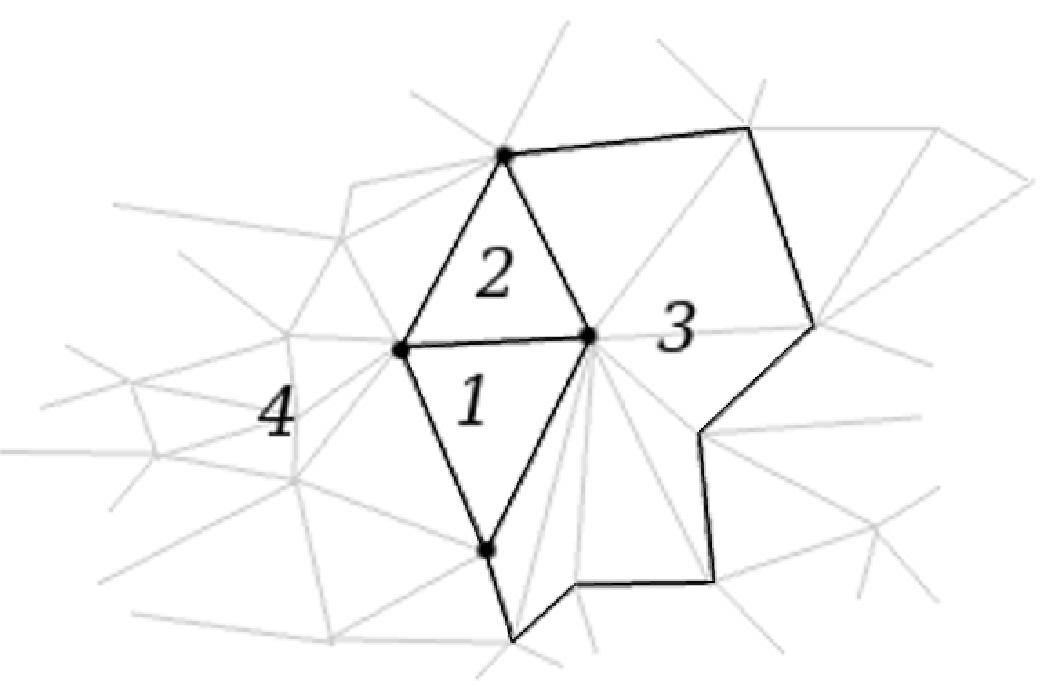
\includegraphics[width=\textwidth]{pseudo-face_pseudo-edge_decomposition.png}
\caption{A simple decomposition of a manifold $\mathcal{M}$ into 4
  pseudo-faces and corresponding pseudo-edges, where $\mathcal{M}$ is
  homeomorphic to the 2-sphere. Figure by David Kamensky.}
\label{fig:pseudo-face-decomposition}
\end{center}
\end{figure}

The algorithm for generating pseudo-faces and pseudo-edges does not
have to be very clever, since Monte Carlo simulations are simulation
independent if we wait long enough, and since the configuration is
immediately randomized (although the the space-like simplices on the
boundary must remain fixed). David's algorithm is as follows:
\begin{enumerate}
\item Select a random triangle in the boundary as the first pseudo-face.
\item Select a random neighbor of the first triangle as a second
  pseudo-face.
\item Select one endpoint of the shared edge between the two triangles
  and let all other triangles that contain that endpoint as a vertex
  be the third pseudo-face.
\item Let all remaining triangles be the fourth pseudo-face.
\item Since each of the first two triangles is a pseudo-face, each
  edge contained by either of those two triangles is a
  pseudo-edge. The sixth pseudo-edge is the combination of edges
  required to completely bound the third pseudo-edge.
\end{enumerate}
Figure \ref{fig:pseudo-face-decomposition} shows this decomposition.
This part of the algorithm is handled by
\textbf{get-s2-pseudo-faces-and-edges}.

The advantage of this approach is that the pseudo-faces and
pseudo-edges meet each other with the same combinatorics as for a
tetrahedron. In this case, we can replace the simplices used to
connect two space-like tetrahedra with analogous complices constructed
of many simplices. Space-like triangles are replaced by pseudo-faces,
space-like edges are replaced by pseudo-edges, and time-like triangles
are replaced by ``triangle fans'' which connect every vertex in a
pseudo edge to a single vertex on the other time slice. The result is
that we have 3 types of complices analogous to the 3 types of
3-simplex, as shown in figure \ref{fig:pseudo-face-complices}. Indeed,
the $(3,1)$-complex can be constructed entirely out of
$(1,3)$-simplices, the $(2,2)$-complex can be constructed entirely out
of $(2,2)$-simplices, and the $(3,1)$-complex can be constructed
entirely out of $(3,1)$-simplices. This information is hard-coded into
the program in the functions \textbf{triangulate-13-complex},
\textbf{triangulate-22-complex}, and
\textbf{triangulate-31-complex}. Each takes in the appropriate
combination of pseudo-faces and pseudo-edges as input, as well as the
low and high time-slice indices as input.

\begin{figure}[htb]
  \centering
  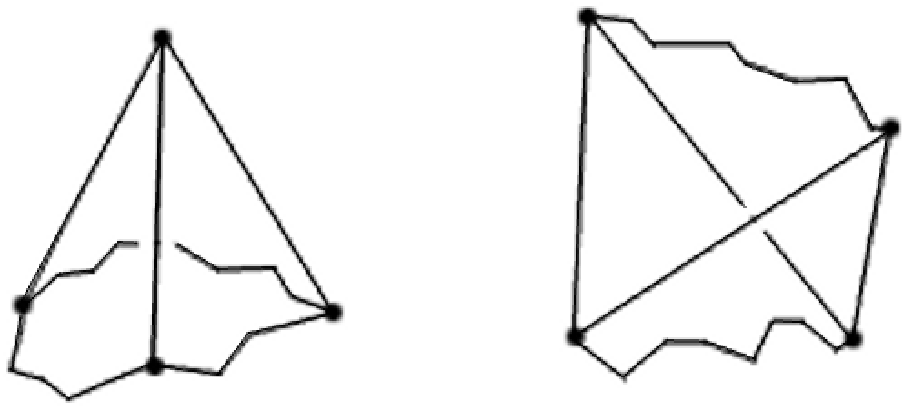
\includegraphics[width=\textwidth]{pseudo-face_complices.png}
  \caption{Possible types of complices constructed by pseudo-faces and
    pseudo-edges. Left: a $(3,1)$-complex. Right: a
    $(2,2)$-complex. The jagged lines are space-like pseudo-edges and
    the straight lines are time-like edges. Figure by David Kamensky.}
  \label{fig:pseudo-face-complices}
\end{figure}

\subsubsection{Generating a Random Spacetime of The Appropriate Size}
\label{sec:grow-spacetime}

Once a minimally triangulated spacetime has been created, as described
in the sections above, we need to generate a spacetime of the proper
3-volume. To do this, use either \textbf{increase-volume-v1} or
\textbf{increase-volume-v2}. By default, the program calls
increase-volume-v2. increase-volume-v1 was written by Christian
Anderson, wile increase-volume-v2 was written by Rajesh
Kommu.
\begin{itemize}
\item increase-volume-v1 has the following prototype:
\begin{lstlisting}
(defun increase-volume-v1 (target-volume))
\end{lstlisting}
  It randomly chooses one of the volume increasing moves until the
  spacetime reaches the target volume, which it takes as input. The
  range of the local variable type-chooser decides the weight and
  frequency of the volume-increasing moves. The advantage of
  increase-volume-v1 is that it is more random than
  increase-volume-v2.
\item increase-volume-v2 has the following prototype:
\begin{lstlisting}
(defun increase-volume-v2 (target-volume))
\end{lstlisting}
  It performs the following algorithm:
  \subitem ---Apply 2-$>$3 moves on all simplices for which this is
  topologically acceptable. 
  \subitem ---Apply 4-$>$4 moves on all simplices for which this is 
  topologically acceptable.
  \subitem ---Apply 2-$>$6 moves on all simplices for which this is 
  topologically acceptable.
  \subitem ---Apply 4-$>$4 moves on all simplices for which this is 
  topologically acceptable.
  \subitem ---Repeat until the total number of 3-simplices in the spacetime 
  is equal to \subitem $\quad$target-volume
\end{itemize}
The advantage of increase-volume-v2 is that it generates an extremely
even volume distribution to start the simulation with before
thermalization. I personally believe this makes thermalization go
faster because the spacetime is probably not in a meta-stable state
to start.

This pretty much covers how to initialize a
spacetime. initialize-t2-triangulation works very much like
initialize-s2-triangulation and calls the same lower-level
functions. However, initialize-t2-triangulation does not support fixed
boundaries.

\subsubsection{Loading a Spacetime From File}
\label{sec:load-from-file}

Instead of initializing (and then probably thermalizing) a new
spacetime, you may wish to load a spacetime from a previous *.3sx2p1
file. The function to call is \textbf{load-spacetime-from-file}, and
has the following prototype:
\begin{lstlisting}
(defun load-spacetime-from-file (infile)
  (parse-parameters-line (read-line infile nil))
  (loop for line = (read-line infile nil)
     while line do (parse-simplex-data-line line)))
\end{lstlisting}
infile is a file stream, not a file name. Therefore, the syntax is :
\begin{lstlisting}[numbers=left]
(defparameter *filename* "/path/to/your/file.3sx2p1")
(with-open-file (f *filename*)
  (load-spacetime-from-file f))
\end{lstlisting}
This function reads a file and generates all 3-simplices defined in
the *.3sx2p1 file and all subsimplices---the function it calls for
this is \textbf{parse-simplex-data-line}. Furthermore, all the
required parameters such as the number of sweeps so far performed, the
number of simplices of each type, and the coupling constants are all
defined---the function it calls for this is
\textbf{parse-parameters-line}.


\subsection{Output Functions}
\label{subsec:output}

Once you've run a simulation, you probably want to see the output. A
catalog of the various data-taking functions is given in the user's
guide, so I won't dwell much on the top-level functions. Instead, I'd
like to talk about how the output functions work and on what
lower-level functions the top-level functions depend on. The
\textbf{generate-data} functions use the following algorithm:
\begin{enumerate}
\item Make the files that are appended to during data creation. See
  section \ref{sec:output-new-files}.
\item Run a Monte Carlo Sweep. See section \ref{s:f:metropolis:loop}.
\item If the sweep number is an integer multiple of
  SAVE-EVERY-N-SWEEPS, append to the files created in step 1 (see
  section \ref{sec:output:appending-to-files}) and make any files that
  are generated anew during data creation (see section
  \ref{sec:output-new-files}).
\item Go back to step 2.
\end{enumerate}

Let's talk about the individual steps in the algorithm. All of the
higher-level functions can be found in \textbf{output.lisp}

\subsubsection{Making new files}
\label{sec:output-new-files}

The functions that generate new files are:

\begin{itemize}
\item \textbf{make-spacetime-file}, which makes *.3sx2p1 files. It
  uses: 
  \subitem \textbf{save-spacetime-to-file}, which prints
  3-simplex information and parameter information to a stream (found
  in \textbf{simplex.lisp}).
\item \textbf{make-progress-file}, which makes *.prg2p1 files.
\item \textbf{make-movie-file}, which makes *.mov2p1 files. It uses:
  \subitem \textbf{print-movie-data}, which is described in section
  \ref{sec:output:appending-to-files}.
\end{itemize}

These functions generate a filename and then print the appropriate
information into the file. Filename generation is handled by a pair of
functions and a battery of constants. The functions are:
\begin{itemize}
\item \textbf{generate-filename}: generate-filename lists a number of
parameters for the simulation, but doesn't specify how many sweeps
have been performed. It is, in general, for generating a single file
over the course of the simulation.
\item \textbf{generate-filename-v2}: generate-filename-v2 works like
  generate-filename, but it keeps track of how many sweeps have been
  performed in the simulation when filename is generated. This is
  useful for generating files periodically during a simulation.
\end{itemize}
The generate-filename functions only generate the bulk of the file
name. The extension is predefined in one of 4 global variables (all of
which are defined in globals.lisp). The extensions are:
\begin{lstlisting}
(defparameter 3SXEXT ".3sx2p1" 
  "used for storing the parameters and 3simplex information")
(defparameter PRGEXT ".prg2p1" 
  "used for keeping track of the progress of a simulation run")
(defparameter MOVEXT ".mov2p1" 
  "used for storing the movie data information")
(defparameter S2SXEXT ".s2sx2p1" 
  "used for storing the spatial 2-simplex information")
\end{lstlisting}

\subsubsection{Appending to Files}
\label{sec:output:appending-to-files}

The only file to which information is appended is a movie data file,
*.mov2p1. We append to a *.mov2p1 file with
\textbf{append-to-movie-file}, which calls \textbf{print-movie-data}
to format the movie data. print-movie-data looks through each
sandwich, counts the number of 3-simplices in that sandwich, and
prints that information to a stream. 

\section{Final Thoughts and TODO}

That about covers the bulk of functions and variables in our current
implementation of fixed-boundaries, 2+1-dimensional CDT. There are
some things I haven't covered, but I hope that the holes are minor and
that it should be relatively easy to figure out how to manipulate the
code that's not discussed.

What's next? Well, in some sense, that's up to you. However, some
obvious gaps are:
\begin{itemize}
\item Fixed boundaries do not function for toroidal spatial
  topologies. It would be nice to extend David Kamensky's algorithm
  for pseudo-faces and pseudo-edges and apply it to the T2 spatial
  topology.
\item Christian Anderson developed a version of the CDT code that can
  incorporate Horava-Lifshitz gravity. Merging the two code bases is a
  daunting task, but I think it would be very much
  worthwhile. Hopefully this programmer's guide would make such a task
  easier.
\item Generating arbitrary boundaries to use with this program is
  non-trivial. I am currently working on a Monte Carlo-inspired method
  in python. The program is called sphere\_generator, and it is almost
  done. Hopefully I'll be finished sometime (relatively) soon.
\item Currently the CDT code-base is not object oriented. However, I
  really think that, with so many people working on the code,
  object-oriented methods could be very helpful. If the data
  structures were objects (which is very natural for geometric objects
  anyway), much less would have to change each time the program is
  modified. LISP has a powerful object oriented library called the
  Common Lisp Object System (CLOS). I think integrating CLOS would
  make editing the code much easier, although there might be a large
  cost in efficiency, which might be why Rajesh didn't include it in
  the first place. In performance computing, ease of coding is often
  sacrificed for speed. Many of Rajesh's algorithms are likely much
  faster than the object-oriented way. For this reason, perhaps
  object-oriented is not a good choice. I guess it's up to you!
\end{itemize}

That's about it. I'd like to thank Rajesh Kommu, David Kamensky, and
Christian Anderson for their previous contributions to the code. I'd
also like to thank Josh Cooperman and Professor Steve Carlip for their
help and guidance on this project.\\
\\
Happy hacking!

\end{document}
